\chapter{Análisis de Resultados}
\section{Resultados}

Se ha logrado mediante la implementación de un sistema de inversor de voltaje alcanzar voltajes de hasta 3.8 KV a una potencia de 20w, voltaje controlado digitalmente por un computador o de manera manual mediante una interface digital. Se ha desarrollado un código en root CERN para encontrar el voltaje RMS de nuestro voltaje de salida. Nuestras mediciones realizadas arrojaron las  distribuciones de las figuras 3.28, 3.29, 3.30 y 3.31 para diferentes voltajes sin carga. \\.


Como observamos se han obtenido voltajes sin perturbaciones y con relativo bajo rizo asociado a él, menor al 1$\%$. Se realizaron cien mil mediciones por cada distribución y a partir de ella podemos observar un voltaje RMS de 4.3V a 93V, este presenta el mayor rizo, ya que nuestro transformador esta diseñado para manejar altos voltajes, 0.00027V para 200V, 0.0011V para 600V y 0.0024V para 986V respectivamente. \\

Se observa en la tabla los siguientes resultados de nuestras mediciones con sus variables correspondientes, siendo bastante obvio que nuestro osciloscopio no logro obtener de manera adecuada las variaciones en voltaje que necesitamos para nuestro análisis. 

\begin{table}[H]
\begin{tabular}{@{}llll@{}}
\toprule
Voltaje   & Frecuencia & Dutty (\%) & Rizo (\%)\\ \midrule
93  & 4.4 KHz        & 4   & $0.043\pm 0.38$\\
200 & 4.05 KHz        & 4   &   $135\mu\pm 0.78$ \\
600 & 4.68 KHz        & 6   &   $185\mu\pm 2.34$ \\
986 & 3.14 KHz       & 7   &   $246.7 \mu \pm 3.85$ \\ \bottomrule
\end{tabular}
\end{table}


\subsection{Análisis espectral} 

Una de las pruebas realizadas a la fuente de alto voltaje para caracterizar su comportamiento fue realizar un análisis de frecuencias. Para esto configuro el PWM a 8KHz y un ciclo de trabajo del 8$\%$, consiguiendo así un voltaje de salida de 300V, para medir de forma segura utilizamos un divisor de voltaje y reducimos el voltaje a 40V. En la figura 3.34 se observa la señal de CD en la parte superior y en la parte inferior el espectro de frecuencias obtenidos, observamos un pico predominante en 0Hz y una serie de picos en frecuencias múltiplos de 8KHz, es decir, la señal cuadra del inversor pasa a través del arreglo de diodos y capacitores del multiplicador del voltaje.

\begin{figure}[H]
\centering
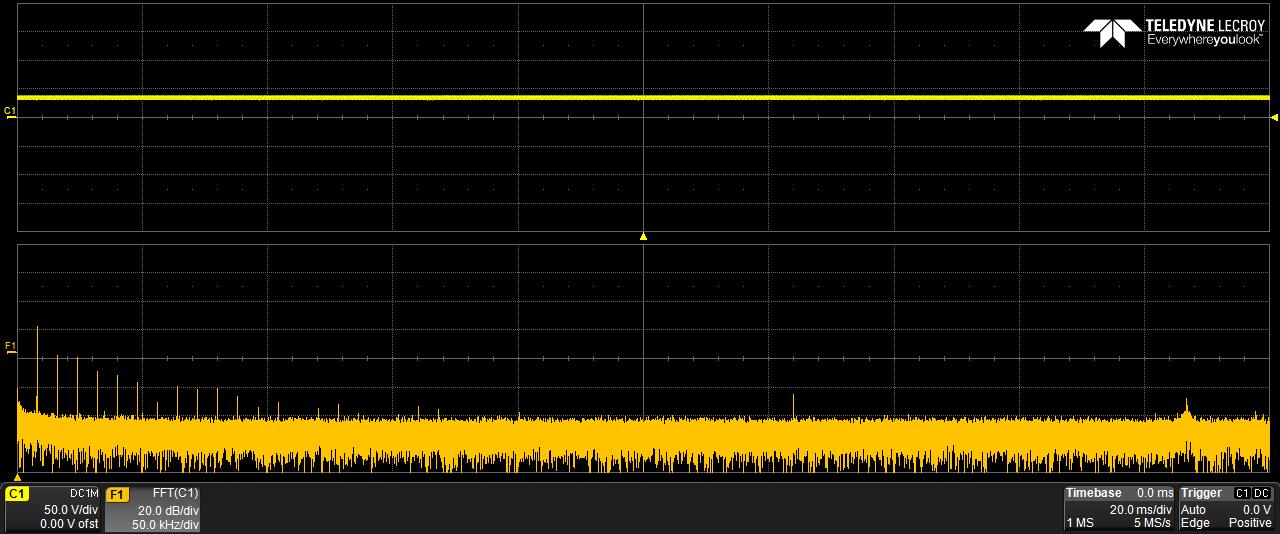
\includegraphics[width=12cm]{Capitulo3/figs/four.jpg}
\caption{Medición sin carga a 986V con un error de 3.85V}
\end{figure}

Es importante mencionar que se hicieron pruebas a bajo voltaje para sacar provecho de los 8 bits de resolución del osciloscopio, cuando subimos el voltaje alrededor de 1kV o 1.5kV (recordemos que el osciloscopio soporta 400Vp de entrada, extendidos a 1.5kV utilizando la sonda del fabricante) la resolución del osciloscopio limita los cambios de voltaje que podemos detectar, en estos casos las mediciones eran muy similares a la siguiente gráfica. En la figura 3.35 observamos la señal de alto voltaje, en la figura 3.36 hacemos un acercamiento a dicha señal, aquí podemos percatarnos que la adquisición solo podía leer dos valores diferentes, es decir, debido a la resolución de nuestro instrumento de medición, solo medimos dos valores de voltaje de toda la componente de rizo de la señal. 

\begin{figure}[H]
\centering
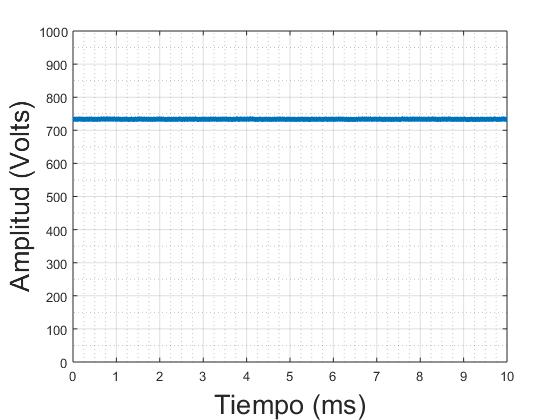
\includegraphics[width=9cm]{Capitulo3/figs/MS.jpg}
\caption{Medición de alto voltaje. }
\end{figure}

\begin{figure}[H]
\centering
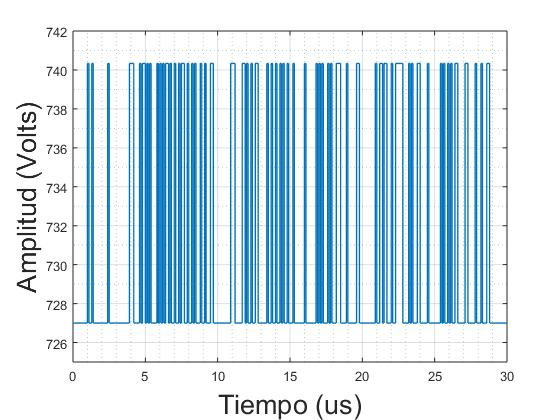
\includegraphics[width=9cm]{Capitulo3/figs/US.jpg}
\caption{Zoom a señal de alto voltaje.}
\end{figure}

\begin{figure}[H]
\centering
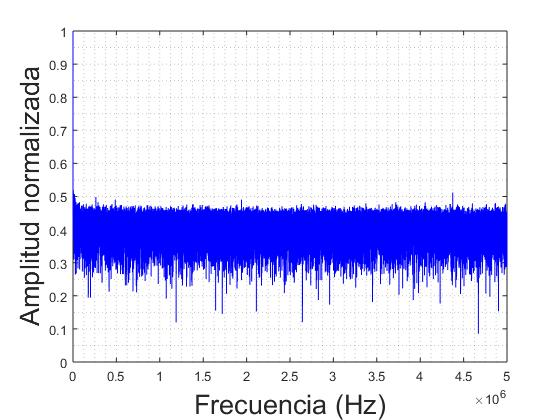
\includegraphics[width=9cm]{Capitulo3/figs/106.jpg}
\caption{Transformada de fourier a señal de alto voltaje.}
\end{figure}

\begin{figure}[H]
\centering
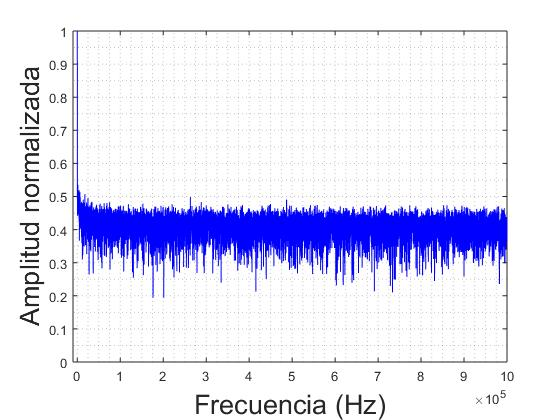
\includegraphics[width=9cm]{Capitulo3/figs/105.jpg}
\caption{Transformada de fourier a señal de alto voltaje desplazada para observar frecuencias en 0 Hz.}
\end{figure}


En la figura 3.37 podemos observar la Transformada de Fourier de la señal de alto voltaje, se observa que no existen componentes importantes salvo en el inicio de la gráfica. En la figura 3.38 podemos observar un acercamiento a la gráfica de la Transformada de Fourier (hasta 1 MHz), como mencionamos anteriormente, solo aparece un pico en 0Hz, el correspondiente al nivel de CD.\\


Para lograr analizar las frecuencias de la señal de ruido apropiadamente, se realizaron mediciones utilizando un acoplamiento a capacitor (10nF) para suprimir la componente de CD y muestrear solamente la AC. En la figura 3.39 observamos la componente de alterna y en la figura 3.40 la Transformada Rápida de Fourier de dicha señal, observamos una diferencia significativa contra el análisis de la gráfica anterior. Observamos una componente fuerte en 0 Hz y otra alrededor de 4.8MHz, aunque la parte mas importante y que se esperaba son frecuencias múltiplos de la señal del inversor, en las figuras 3.41 y 3.42 observamos componentes en 500 Hz, 1Khz, 1.5Khz, 2KHz, etc. La señal del inversor para esta prueba fue de 500Hz y un ciclo de trabajo de 5%. 


\begin{figure}[H]
\centering
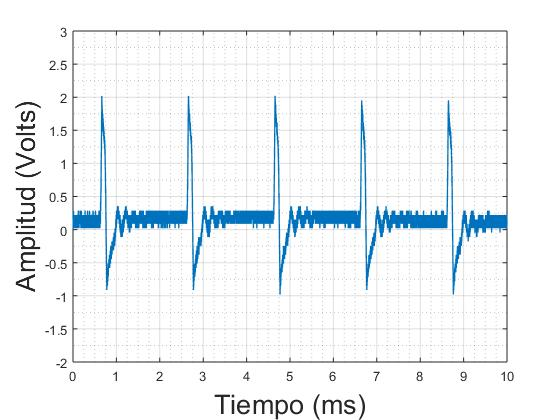
\includegraphics[width=9cm]{Capitulo3/figs/reso.jpg}
\caption{Zoom de voltaje acoplado a capacitor.}
\end{figure}

\begin{figure}[H]
\centering
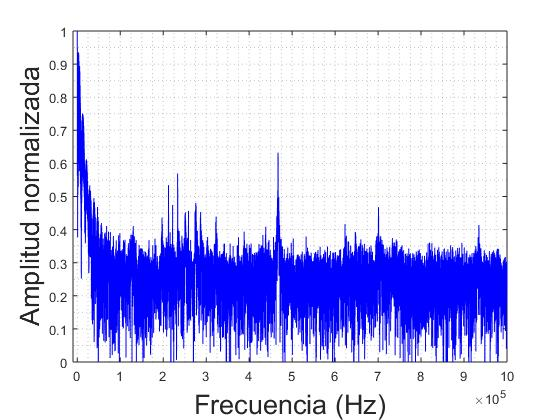
\includegraphics[width=9cm]{Capitulo3/figs/X105.jpg}
\caption{Transformada de fourier de señal de voltaje acoplado a un capacitor. 100 KHz por división.}
\end{figure}

\begin{figure}[H]
\centering
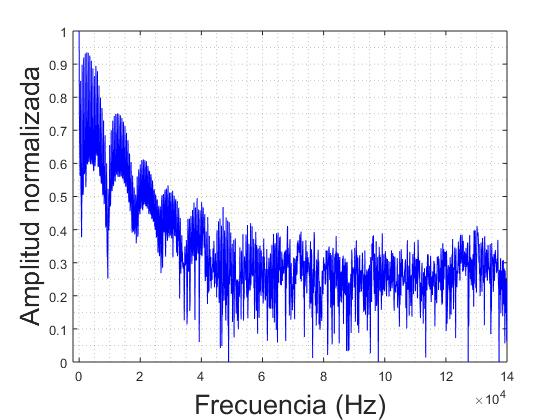
\includegraphics[width=9cm]{Capitulo3/figs/reso2.jpg}
\caption{Transformada de fourier de señal de voltaje acoplado a un capacitor. 10 KHz por división.}
\end{figure}

\begin{figure}[H]
\centering
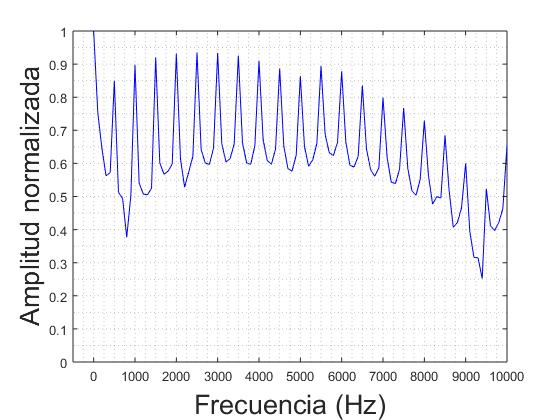
\includegraphics[width=9cm]{Capitulo3/figs/KHZ.jpg}
\caption{Transformada de fourier de señal de voltaje acoplado a un capacitor. 1 KHz por división.}
\end{figure}


Los resultados indican que se ha desarrollado una fuente que ha logrado superar los 3.8 KV, encontrando limitado nuestro análisis del ruido por la resolución de nuestras herramientas de medición, obteniendo una amplitud del riso en el orden de los 3 V pico-pico con la anterior configuración. Este riso corresponde al  0.375$\%$ de la señal. \\
